\documentclass[12pt]{article}
\usepackage[a4paper, total={7in, 8in}]{geometry}
\usepackage{graphicx,amssymb,dsfont,fourier,xcolor,amsmath,ulem,filecontents,MnSymbol,wasysym}
\usepackage[utf8]{inputenc}

\title{Heat Exchanger Simulation Report: TP1}
\author{User}
\date{29.04.2025}

\begin{document}
\maketitle
\tableofcontents

\section{Introduction}
This report presents the results of the TP1 simulation for a heat exchanger.

\section{Experimental Parameters}
\begin{itemize}
    \setlength\itemsep{-0.5em}
    \item Cold Fluid: water
    \item Hot Fluid: water
    \item Material: stainless steel
    \item Cold Inlet Temperature: 20°C
    \item Hot Inlet Temperature: 80°C
    \item Pipe Length: 2 m
    \item Pipe Diameter: 0.1 m
\end{itemize}\n
\section{Methodology}
The simulation uses the following heat transfer equations:
\begin{equation}\label{eq:tp1_heat_transfer}

    Q = \dot{m} \cdot c_p \cdot (T_{out} - T_{in}) \quad \text{(Heat transfer)} \\
    Q = U \cdot A \cdot \Delta T_{lm} \quad \text{(Overall heat transfer)}
    
\end{equation}\n
\section{Results and Discussion}
\begin{figure}[htb!]
        \centering
        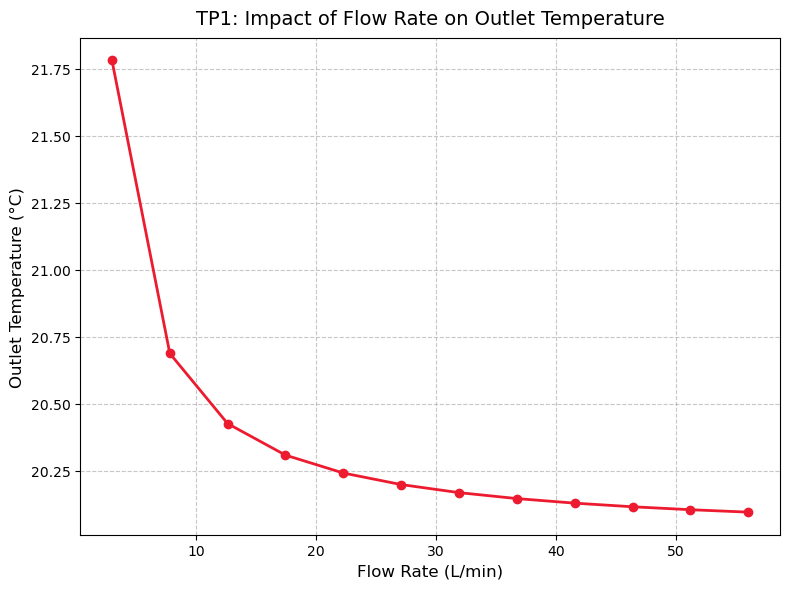
\includegraphics[width=0.8\textwidth]{tp1_plot.png}
        \caption{Simulation results for TP1}
        \label{fig:tp1_results}
\end{figure}\n\begin{table}[ht!]
        \centering
        \begin{tabular}{|l|c|c|c|}
\hline
Flow Rate (L/min) & Outlet Temp (°C) & Heat Transferred (W) & Efficiency (%) \\
\hline
5.0 & 29.09 & 3170.16 & 15.15 \\
\hline
13.636363636363637 & 23.51 & 3341.27 & 5.85 \\
\hline
22.272727272727273 & 22.18 & 3381.43 & 3.63 \\
\hline
30.90909090909091 & 21.58 & 3399.36 & 2.63 \\
\hline
39.54545454545455 & 21.24 & 3409.52 & 2.06 \\
\hline
48.18181818181819 & 21.02 & 3416.06 & 1.69 \\
\hline
56.81818181818182 & 20.86 & 3420.62 & 1.44 \\
\hline
65.45454545454545 & 20.75 & 3423.98 & 1.25 \\
\hline
74.0909090909091 & 20.66 & 3426.56 & 1.1 \\
\hline
82.72727272727273 & 20.59 & 3428.6 & 0.99 \\
\hline
91.36363636363637 & 20.54 & 3430.26 & 0.9 \\
\hline
100.0 & 20.49 & 3431.64 & 0.82 \\
\hline
\end{tabular}
        \caption{Results for TP1: Flow Impact}
        \label{tab:tp1_results}
\end{table}\n
\section{Conclusion}
The simulation results show the impact of the varied parameter on the outlet temperature, heat transferred, and efficiency.

\end{document}
